\chapter{Le site web de l'association \ofni}
\label{chap:site}

Le but de ce projet est de réaliser le site internet de l'association \ofni.

\section{Le projet}

Ce rapport présente le développement que nous avons réalisé dans le cadre du projet tutoré de troisième année de Licence Informatique à l'\univ\ de \propre{Besançon}.
\bigskip

Le sujet de ce projet était de développer un site \web\ pour une association étudiante, en équipe de trois personnes. L'objectif était de mobiliser nos compétences en développement \web\ tout en en acquérant de nouvelles.

Pour cela, nous avons été encadrés par Monsieur \nom{Alexandre}{Demougin} et Madame \nom{Alicia}{Pierrot}, depuis la conception du site jusqu'à sa mise en ligne, ainsi que pour la rédaction de ce rapport et la préparation de notre soutenance orale.
\bigskip

Nous avions quelques mois pour mener à bien ce projet, qui était divisé en trois grandes phases:

La première, de novembre à décembre 2024, portait sur la phase de conception et de maquettage du site. 
Celle-ci consistait dans un premier temps à trouver les fonctionnalités du site ainsi que les besoins auxquels il devait répondre. 
Dans un second temps, cette phase consistait en l'élaboration de la maquette du site, contenant l'entièreté des pages du site ainsi que leurs visuels.

La seconde étape, de janvier à février, était la phase de développement du site. 
Celle-ci correspondait à une période de recherche et de réflexion sur les technologies existantes, le choix des plus adaptées pour la réalisation du projet, ainsi que le développement et le codage du site.

Enfin, la dernière phase, de février à mars, était la phase de réalisation de ce rapport et de la soutenance orale.

\section{L'association \ofni}

Fondée en 1997, l'\ofni\ est l'association des étudiants en informatique de l'\univ\ de \propre{Besançon}.
\bigskip

L'association a pour but de rassembler les étudiants des différentes promotions autour d'activités communes (sorties, barbecues, Nuit de l'Info, etc.) et de favoriser l'entraide entre promotions.

L'\ofni\ joue également un rôle d’intermédiaire entre ses membres, les chercheurs et les entreprises en maintenant un réseau d’anciens étudiants et des contacts avec ses sponsors.
\bigskip

Le projet restait lible sur le choix de l'association et des technologies utilisées.
C'est en équipe que nous avons choisi de réaliser le site de l'association \ofni{}. 
Notre équipe faisant partie du bureau actuel de l'association, notre choix s'est donc imposé naturellement. 
Bien que l'association avait déjà un site, celui-ci était obsolète et ne répondait plus aux besoins actuels de l'association, comme le montre la \figureref{oldsite}.
De plus, il n'était plus maintenu et présentait des failles de sécurité.
\bigskip

\begin{figure}[!ht]
    \centering% 
    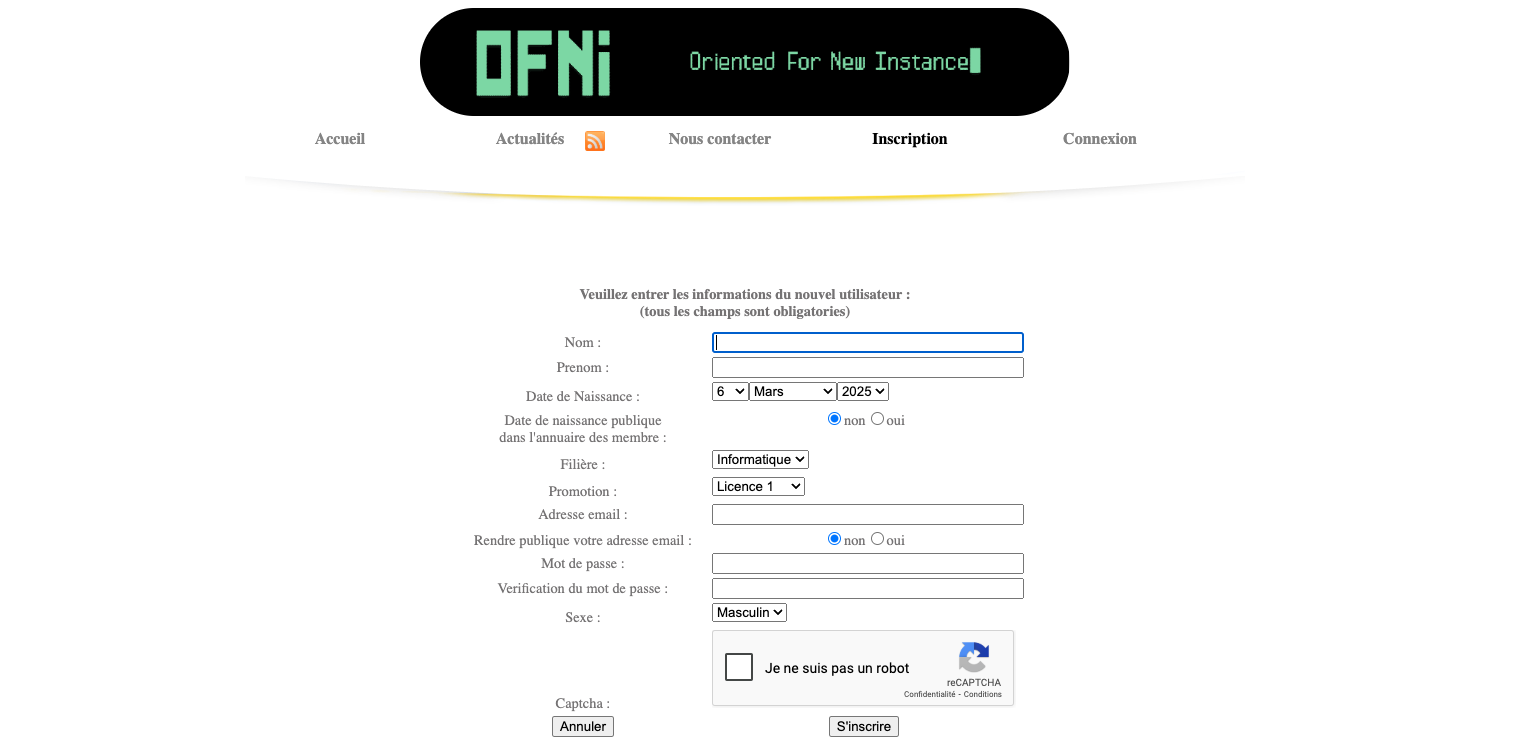
\includegraphics[width=15cm]{assets/pictures/old-site.png}
    \caption[\emph{Ancien site de l'association \ofni}]{Ancien site de l'association \ofni}%
    \label{oldsite}%
\end{figure}
\bigskip

Les consignes sur la réalisation du site étaient de créer une interface claire et intuitive, de développer une solution robuste et fonctionnelle, le tout en mettant l’accent sur l’efficacité et la maintenabilité du site.
\bigskip

Les fonctionnalités envisagées incluaient la présentation des activités de l’association, une vitrine pour les projets étudiants, la possibilité de réaliser des sondages pour les événements et la mise à disposition d’informations pour les lycéens souhaitant découvrir l’association.
